\chapter{Introduction}
\label{chap:intro}

Distributed systems are widely used
  in everything from web infrastructure to airplanes,
  and their correctness is critical.
These systems are notoriously hard to implement correctly
  because they are expected to tolerate execution in harsh environments,
  where concurrency and partial failure are a fact of life,
  all while no single node has access to a global view of the system state.
Traditional testing techniques are inadequate
  for exploring the space of possible executions
  in the presence of concurrency and partial failure
  because this space includes the exponential number of
  interleavings of system events and failure events.
Furthermore, even considering a particular interleaving of events,
  one faces all the usual difficulties with testing a sequential program,
  including the issue of achieving sufficient coverage.

Since testing is not enough for distributed systems,
  the research community has developed
  a rich body of work applying formal methods
  to exhaustively check correctness.
Applying formal methods is not a panacea, however,
  because complex systems have complex proofs of correctness.
It is not uncommon, \eg,
  for a  distributed file system to coordinate thousands of machines
  using a combination of several different protocols to ensure
  consistency, fault tolerance, and high performance.
The primary challenge to applying verification to distributed systems is
  high system complexity, which leads to high proof complexity.
To verify a system such as a distributed file system,
  one must break the problem down into smaller parts.
In the face of high system complexity,
  decomposing the problem reduces proof complexity and increases automation.
Decomposing proofs leads to two benefits.
First, a truly compositional proof
  imposes no additional proof burden
  to put the pieces back together.
Second, sufficiently decomposed pieces can
  be analyzed fully automatically using decision procedures.

The central claim of this dissertation is:
\begin{center}
\emph{Programming languages techniques for compositionality
  lay the foundations for effective, automated verification of
  distributed systems implementations.
}
\end{center}

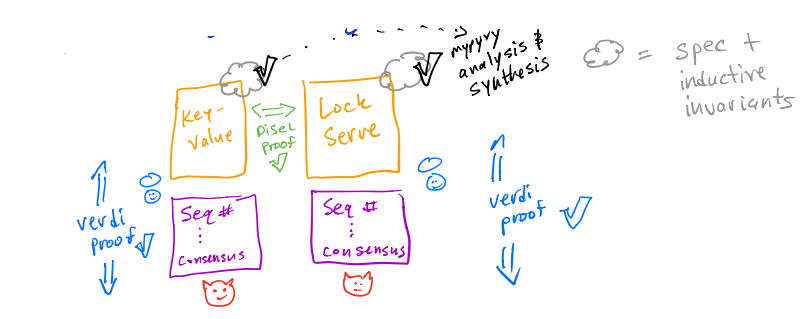
\includegraphics[width=\textwidth]{intro-cartoon.png}

The remainder of this dissertation addresses three challenges in system complexity
  by applying programming languages techniques to decompose the problem,
  thus increasing automation and decreasing proof complexity.

\Cref{chap:verdi} addresses complexity challenges due to fault tolerance
  by introducing Verdi,
  a \Coq~\cite{Coq} framework for implementing and verifying distributed systems
  that supports compositional fault tolerance reasoning
  through \emph{verified system transformers}.
Verdi models system execution using various \emph{network semantics},
  each of which encodes assumptions about the environment
  including possible network faults and machine failures.
Network semantics can range from the idealistic to the pessimistic.
For example, one might assume that
  all messages are eventually delivered and that nodes never fail.
On the other hand, one might assume that
  packets can be dropped and duplicated and that
  some nodes behave arbitrarily or maliciously.
Different systems are designed under different sets of assumptions,
  and network semantics capture those assumptions.
The main point of defining a particular network semantics in Verdi is
  to verify distributed systems using that semantics as the fault model.
Assuming the network semantics accurately describes
  all possible behaviors of the system's environment,
  a proof in Verdi guarantees that the system is correct for all executions.
For common network semantics,
  there are typically generic mechanisms that systems use to tolerate faults,
  \eg, sequence numbering to handle message reordering and duplication.
Another key benefit of
  clearly stating environment assumptions as network semantics is that
  one can then express these generic fault tolerance mechanisms
  as transformers between semantics.
Using transformers, the engineer can
  implement and reason about their application
  in a fault model with relatively few faults, and
  then automatically transform the system into one
  that provably works in a more adversarial fault model
  with relatively more faults.
We used Verdi to study the Raft consensus protocol~\cite{ongaro:raft},
  producing the first formal proof of safety
  and the first verified implementation.
The Verdi framework was originally described in a PLDI 15 paper~\cite{Wilcox-al:PLDI15},
  and an extended case study proving
  the safety of the Raft consensus protocol was published in CPP 16~\cite{Woos-al:CPP16}.
These papers were written together with a fantastic team of coauthors:
  Doug Woos, Pavel Panchekha, Steve Anton, Zachary Tatlock, Xi Wang, Michael D.\ Ernst, and Thomas Anderson.
\Cref{chap:verdi} is a combined narrative of these two papers with minor improvements.
The Verdi code is publicly available at \url{https://github.com/uwplse/verdi}.

%whose key insight is to treat the network as analogous to the heap in
%sequential programming.


\Cref{chap:disel} details \disel,
  a concurrent separation logic for distributed systems.
Whereas
  Verdi separates fault tolerance reasoning from application logic
  (which we call vertical compositionality),
  \disel separates reasoning about cooperating services
  by defining interfaces that capture protocol-specific invariants
  (which we call horizontal compositionality).
This supports verifying modern distributed systems
  which are typically built by composing several services
  to provide a high-level application.
A proof of correctness for a system composed of several services
  should similarly compose the guarantees of each individual service.
Using the techniques of Verdi alone,
  such reasoning is not possible.
Instead of reasoning across fault models,
  what we need is
  to abstract over the low-level details
  each component uses to provide its guarantee.
To achieve this, we take inspiration
  from modern program logics for concurrent programs
  that manipulate heap pointers.
These logics allow modular reasoning
  by separating different parts of the heap,
  each of which can be reasoned about independently.
\disel applies this insight to distributed systems
  by analogizing the network as the heap.
Thus, \disel separates the network messages
  of each protocol from each other,
  allowing independent reasoning.
\disel achieves this through several logical mechanisms
  that support strengthening the invariants
  of other services with client-specific facts and
  capturing the essential interactions
  between protocols with \emph{hooks},
  which allow one protocol's actions
  to be conditioned on another protocol's state.
\disel was originally published in SNAPL 17 and POPL 18~\cite{Wilcox-al:SNAPL17, disel-popl18},
  and would not have been possible without my wonderful collaborators,
  Ilya Sergey, Zachary Tatlock, and Miranda Edwards.
\Cref{chap:disel} is a polished version of these papers.
The \disel code is publicly available at \url{https://github.com/DistributedComponents/disel}.

Experience in \disel and Verdi showed
  that the manual effort required
  to provide strong guarantees about distributed systems
  doesn't scale with current tooling.
In particular, the key sticking point is developing inductive invariants.
Deductive verification techniques,
  such as those used in \disel and Verdi,
  are highly expressive
  but require the user to provide a great deal of additional input,
  including inductive invariants and their proofs.
For example, using Verdi to prove an application correct
  in a relatively nice fault model
  still requires deriving an application-specific invariant,
  which simultaneously
    (1) summarizes all the reachable states of the application,
    (2) is closed under the transition system's step relation, and
    (3) ensures the absence of safety violations.
The difficulty of deriving these invariants
  inspired us to investigate techniques
  for automatically proving and even \emph{inferring} inductive invariants.

\Cref{chap:mypyvy} describes \mypyvy,
  a tool for automated reasoning
  about symbolic transition systems in first-order logic.
\mypyvy takes an input file
  describing a symbolic transition system
  and can perform a variety analyses, as requested by the user.
Three of the most interesting analyses include
  inductive invariant checking,
  invariant inference, and
  bounded trace reasoning.
In all cases, \mypyvy loads the transition system
  and compiles it together with the user-requested analysis
  to a (sequence of) SMT queries,
  which are dispatched to Z3.
\mypyvy was originally developed to support a CAV 19 paper~\cite{phase-updr},
  but that paper was not about \mypyvy per se.
\Cref{chap:mypyvy} contains previously unpublished material describing \mypyvy itself
  and will become the primary reference for \mypyvy.
The development of \mypyvy has benefited greatly from many contributors,
  especially Oded Padon, Yotam Feldman, Sharon Shoham, Mooly Sagiv, Jason R.\ Koenig,
  Ken McMillan, Alex Aiken, Giuliano Losa,
  Daniel Ricketts, Shachar Itzhaky, Lindsey Kuper, William Schultz, and Aaron Weiss.
\mypyvy is actively developed at \url{https://github.com/wilcoxjay/mypyvy}.

Distributed systems remain a crucial topic
  with many potential avenues for future work.
In \cref{chap:conclusion},
  we summarize our plans
  for extending Verdi, \disel, and \mypyvy
  to further improve the verification experience.
We are especially excited
  to live in a world where more users
  are empowered to verify their distributed systems.